In this chapter, we present the phenomenological results for
\Wbb~production in association with up to three jets at the LHC
$\sqrt{s}=13$ TeV, as shown in Ref.~\cite{wbbpaper}. First, we analyze
effects of a finite $b$-mass by comparing results obtained in both the
four-flavor number (4FNS) and five-flavor number (5FNS)
scheme. Secondly, we present results for total and differential cross
sections and study their renormalization- and factorization-scale
dependence. And lastly, we present a series of
observables associated to $HW$ production measurements and show predictions
of exclusive sums, which combine cross sections of distinct light-jet multiplicities 
and assess
their theoretical uncertainty based on scale dependence, higher-order
contributions and PDF errors. 

\section{Effects of a Finite Bottom-Quark Mass}
\label{sec:bmass}
The effects of a finite $b$ quark mass in \Wbb{} production have been studied since the early NLO QCD
calculations in Ref.~\cite{FebresCordero:2006sj}. We consider situations with two
well defined $b$ jets, where the effects of a finite bottom-quark mass are expected to be small since ratios of invariants involving $m_b^2$ are typically small. However, the effect of a finite $b$ quark mass is important for inclusive $b$-jet
production at hadron colliders (see for example Refs.~\cite{Campbell:2006cu,Campbell:2008hh,Caola:2011pz}).\footnote{Here, only one $b$-jet is required to pass a $p_T$ cut whereas the other $b$-jet remains unrestricted. In some regions of phase space the $b\bar{b}$ jet invariant mass can become not much larger than $2m_b$ and effects of a finite $b$-mass are sizeable.} We leave the study of inclusive $b$-jet production in association with multiple light jets using our matrix elements to future work. 

In this section, we analyze the effects of a finite mass of the bottom quark
$m_b$ in our results. To this end, we compare both total cross-sections and
differential distributions computed in two different schemes. In the
four-flavor number scheme (4FNS) bottom quarks are consistently
treated as massive particles that can appear in the final-state and as virtual particles in loop diagrams. Corresponding PDFs, and the DGLAP
equations to evolve them, consider only four quark flavors ($d$, $u$, $s$ and
$c$) and the gluon as partons. For the 4FNS calculation, we use our default setup (as
described in Section~\ref{sec:base_setup}). We compare to a
computation in the five-flavor number scheme (5FNS), where bottom
quarks are consistently treated as massless particles in the hard scattering matrix
elements. The corresponding PDF sets thus have five quark flavors and the gluon
as partons. 

We perform an analysis for \Wbb{} and \Wbbnj[1]{} production with the aim
of confirming the findings of Ref.~\cite{FebresCordero:2006sj} also
for \Wbbnj[1]{}. Note in particular that apart from real-emission diagrams
for \Wbbnj[1]{}, the considered diagrammatic content is the same in the
4FNS and the 5FNS for both these processes, since no bottom-initiated
diagrams exist. We can thus attribute appearing difference to $b$-mass effects in matrix elements, phase space generation, differences in PDFs and the corresponding running couplings. Given the similar diagrammatic content, it might be interesting in the future to also compare \Wbbnj[2]{}
and \Wbbnj[3]{} production, for which no such
limitation exists, in the two flavor-number schemes. We leave this
more systematic comparison of the 4FNS vs.~5FNS to future work.

The two schemes are characterized by a different organization of the
perturbative series used for computing observables. Given that for
example $\alps^{N_f=4}(M_Z^2)$ has a value of about 0.113 and
$\alps^{N_f=5}(M_Z^2)$ of 0.118, differences between the two
schemes can potentially appear. Nevertheless, we will see that in regions where characteristic scales $Q^2$ are such that the ratios
$m_b^2/Q^2$ are small, we find good agreement at NLO QCD between the
4FNS and the 5FNS. This shows that the differing terms in the perturbative series are small for the
observables considered in this study (a dedicated study of the different
perturbative contributions appearing in these different schemes appeared in
Ref.~\cite{Maltoni:2012pa}).

In our analysis of the 4FNS and 5FNS calculations, we require two $b$ jets and $n$ light jets, as defined by the anti-$k_T$ jet
algorithm~\cite{antikT} with $R=0.4$. We apply the following event
selection cuts, with the same cuts applied to $b$ and light jets
\begin{align}
  p_T^{\text{jet}}&>15\text{ GeV},& |\eta^{\text{jet}}|&<2.4\ ,\notag\\
  p_T^{e}&>25\text{ GeV},& |\eta^{e}|&<2.5\ ,\notag\\
  p_T^{\nu}&>20\text{ GeV},& M_T^W &> 20\text{ GeV}.
  \label{eq:massivemasslessCuts}
\end{align}
We define $b$ jets (in both massive or massless cases) by
quark-flavor content of the jets in an infrared-safe manner according
to~\cite{Banfi:2006hf}. In the 5FNS calculations,
we use PDFs from CT14~\cite{CT14}, denoted by \texttt{CT14llo} at LO and
\texttt{CT14nlo} at NLO and include closed massive top loops. Closed bottom
loops in the 5FNS are computed with massless quarks.

%%%%%%%%%%%%%%%%%%%%%%%%%%%%%%%%%%%%%%%%%%%%%% 
\begin{table}[ht]
  \setlength{\tabcolsep}{1.6pt}
  \small
  \begin{tabular}{@{} c
      @{\hspace*{\lengthd}}     c
      @{\hspace*{\lengthd}}c
      @{\hspace*{\lengthc}}c
      @{\hspace*{\lengthc}}c
      @{\hspace*{\lengthd}}c
      @{\hspace*{\lengthc}}c @{}}
    \hline\hline
    \noalign{\vskip 2.5mm}
    jets  & massive~LO & massive~NLO & $K$-factor & massless~LO & massless~NLO & $K$-factor\\
    \noalign{\vskip 2mm}
    \hline
    \noalign{\vskip 2mm}
    0 & $0.81177(32)^{+0.1379}_{-0.1113}$ &
    $1.6804(20)^{+0.3071}_{-0.2300}$  & $2.07$ &
    $0.95905(41)^{+0.1507}_{-0.1247}$ &
    $2.0051(44)^{+0.3527}_{-0.2673}$  & $2.09$\\
    \noalign{\vskip 2mm}
    1 & $0.96210(93)^{+0.3630}_{-0.2457}$ &
    $1.3748(82)^{+0.2422}_{-0.2200}$  & $1.43$ &
    $1.1756(19)^{+0.4279}_{-0.2940}$ &
    $1.7132(80)^{+0.2907}_{-0.2636}$  & $1.46$\\
    \noalign{\vskip 2mm}    
    \hline\hline
  \end{tabular}
  
  %%%%%%%%%%% TABLE xs  %%%%%%%%%%%%%%%%%%%%%%%%%%

\caption{LO and NLO QCD cross sections for \Wbbm+$0,1$-jet~$+X$ production
within the 4FNS (massive) and the 5FNS (massless). Results with dynamical scale
$\HTpartonicp/2$ are shown together with their respective $K$-factors. Kinematical
cuts are specified in \eqn{eq:massivemasslessCuts}.  The number in
parenthesis next to the central value gives the corresponding statistical
integration error.
Super and subscripts denote scale variations. \label{tab:wcomp_total_xs} }
\end{table}

In Table \ref{tab:wcomp_total_xs} we show the results at the level of total
cross sections as computed in the 4FNS and 5FNS. We observe a clear deviation
between the central results, with the 5FNS results producing total cross
sections about 20\% larger. However, the
structure of the corrections, both by the size of the $K$-factor and by the
scale sensitivity at NLO, is very similar. 



%mbb spectrum Wbb & Wbbj massive/massless
%%%%%%%%%%%%% FIGURE %%%%%%%%%%%%%%%%%%
\begin{figure}[]
\begin{center}
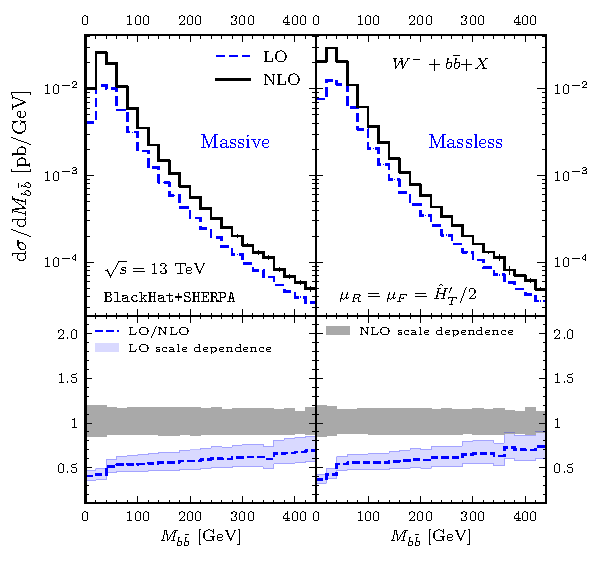
\includegraphics[clip,scale=1]{plots/cmbbwbb}
\end{center}
\begin{center}
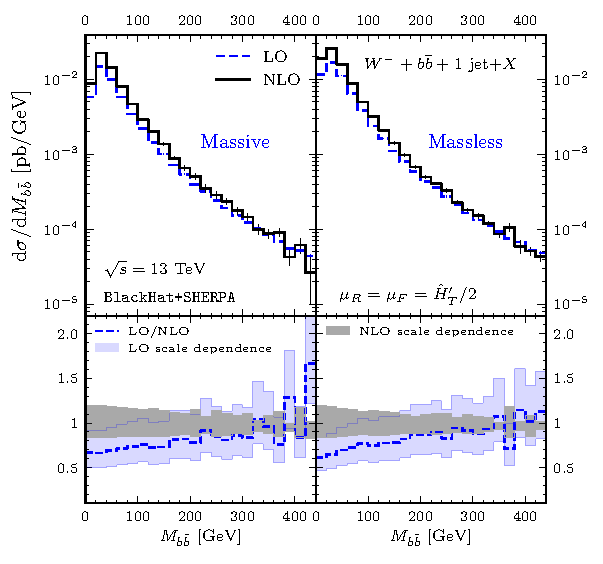
\includegraphics[clip,scale=1]{plots/cmbbwbbj}
\end{center}
\caption{The invariant mass spectra for the $b\bar b$ system in \Wbbm{} (top) and
    \Wbbm+1-jet (bottom) production at the LHC at
    $\sqrt{s}=13$~TeV, for calculations performed at LO and NLO QCD order within
    the 4FNS (left) and the 5FNS (right). In the upper panel of each
    figure, we show the LO (dashed blue line) and NLO (solid black
    line) results with thin vertical
    lines representing the numerical integration errors. The bottom panels show
    the scale-dependence bands normalized to the NLO result in blue for LO and
    gray for NLO.}
  \label{fig:Wmmbb}
\end{figure}
%%%%%%%%%%%%%%%%%%%%%%%%%%%%%%%%%%%%%%%

%mbb spectrum Wbb & Wbbj ratio massive/massless
%%%%%%%%%%%%% FIGURE %%%%%%%%%%%%%%%%%%
\begin{figure}[]
\centering
%\begin{centering}
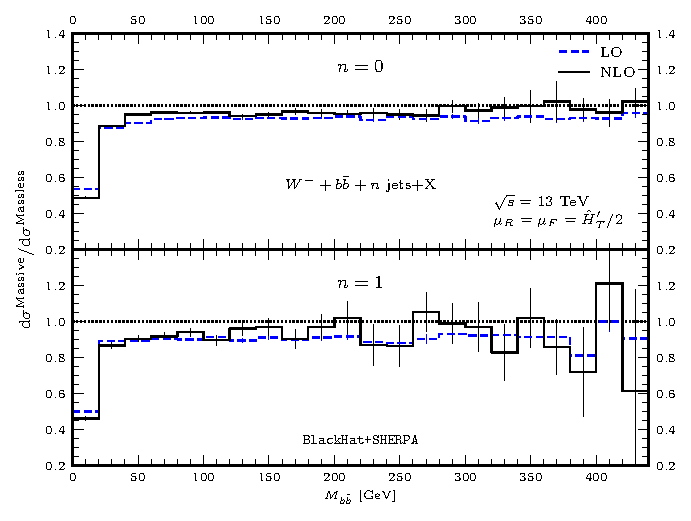
\includegraphics[clip,scale=1.02]{plots/crmbb}
%\end{centering}
  \caption{Ratio of the invariant mass spectrum of the $b\bar b$
    system in a 4FNS calculation to a 5FNS one, for \Wbbm{} (top) and \Wbbm+1-jet (bottom) production. The ratios are taken at LO (dashed blue line) and at NLO (solid black line).
    Statistical errors are shown as thin vertical lines. We include a dotted
    horizontal line at a ratio value of 1.}
  \label{fig:ratWmmbb}
\end{figure}
%%%%%%%%%%%%%%%%%%%%%%%%%%%%%%%%%%%%%%%

In the following, we show that this difference on the level of total cross sections can be largely attributed to regions of phase space in which
$m_b^2$ cannot be considered a small quantity. We do so by looking at the
structure of our results over phase space and find that the effects are
quite similar at LO and at NLO, as originally shown
in~\cite{FebresCordero:2006sj}. In particular, we show distributions in the invariant
mass of the $b\bar b$ system, but similar effects are found for
example for the $p_T$ distributions of the leading and subleading $b$ jets.

In Fig.~\ref{fig:Wmmbb} we show the $M_{b\bar b}$ distribution for \Wbbm{} and
\Wbbm$+1$-jet production computed at LO and NLO in both the 4FNS and
5FNS. \Wbb{} production exhibits large radiative corrections, as
visible in the ratio panels, while the
results for \Wbbnj[1]{} production show less structure over phase space. 


In order to highlight the
differences between the two calculations, we show the ratio of massive
calculation (4FNS) to massless calculation (5FNS) in Fig.~\ref{fig:ratWmmbb}. We notice that the differences observed at the level of the total cross
sections can be mostly attributed to the regions of small $M_{b\bar
  b}$. For values of $M_{b\bar b}$ above 50 GeV, the ratios stabilize rapidly at about
0.95 for \Wbb{} production and at 0.9 for \Wbbnj[1]{} production, whereas
we have a strong deviation for lower values, with the massless
calculation more than doubling the massive one.  The discrepancy is to
be expected, since in these regions,  phase-space constrains the production of massive $b$ quarks and $m_b$
 effects in the matrix elements are noticeable.


 The mass effects are not affected by
quantum corrections, as we can deduce from the similarity of the LO and NLO
ratios. The deviation from 1 at large $M_{b\bar b}$ is smaller than
the scale-dependence bands of the NLO results. Notice that the 4FNS and 5FNS have by
construction different renormalization schemes. Also, it is important
to mention that the intrinsic difference of the global QCD analyses to produce
4FNS and 5FNS PDF sets induce discrepancies both in $\alps$ and the gluon-PDF
that can account for the massless results increase of about 5\% for \Wbb{}
production and of about 10\% for \Wbbnj[1]{} production. The PDF uncertainties
associated to the global QCD analysis are relatively small, at the level of 1 or 2\%
as we will show in Section~\ref{sec:hw}.


%%%%%%%%%%%%%%%%%%%%%%%%%%%%%%%%%%%%%%%%%%%%

\section{Results for \Wbb{} Production in Association with Light Jets}
\label{sec:vjets}
In this section we present NLO QCD results for \Wbb~production in
association with up to three light jets in
$pp$ collisions at the LHC Run-II with $\sqrt{s}=13$ TeV. We show total cross sections and differential distributions as a function of the light-jet multiplicity. We obtain our results by applying the following kinematical cuts
\begin{align}
  p_T^{\text{jet}}&>25\text{ GeV},& |\eta^{\text{jet}}|&<2.4\ ,\notag\\
  p_T^{e}&>25\text{ GeV},& |\eta^{e}|&<2.5\ ,\notag\\
  p_T^{\nu}&>20\text{ GeV},& M_T^W &> 20\text{ GeV}\ ,
  \label{eq:Cuts}
\end{align}
where the same cuts are applied to both light and
$b$ jets. The computational setup is described in Chap.~\ref{chap:wbb_intro} and renormalization and factorization scales are chosen to be equal and are dynamically set to $\mu=\HTpartonicp/2$, according to
Eq.~\eqref{eq:htpart}. Jets are defined by using the
anti-$k_T$ jet algorithm~\cite{antikT} with $R=0.4$, as implemented in the
\texttt{FastJet} package~\cite{Cacciari:2011ma}.

\subsection{Total Cross Sections}
\label{totalxsw}
In Table \ref{tab_Wpj_total_xs}, we present total partonic cross
sections for the inclusive production of
both $W^-$ and $W^+$ accompanied by two $b$ jets and zero to three
light jets. We give the numerical integration uncertainty in
parenthesis and quote the scale dependence in superscripts and subscripts. In separate columns, we show the ratio of NLO to LO results, the so called $K$-factors, which quantify the total size of the NLO corrections.

%%%%%%%%%%%%%%%%%%%%%%%%%%%%%%%%%%%%%%%%%%%%%% 
\begin{table}[ht]
  \small
  \begin{center}
    \begin{tabular}{@{} c
        @{\hspace*{\lengthb}}     c
        @{\hspace*{\lengthb}}c
        @{\hspace*{\lengtha}}c
        @{\hspace*{\lengtha}}c
        @{\hspace*{\lengthb}}c
        @{\hspace*{\lengtha}}c @{}}
        \hline\hline
        \noalign{\vskip 2.5mm}
        jets  & \Wbbm~LO & \Wbbm~NLO & $K$-factor & \Wbbp~LO &
        \Wbbp~NLO & $K$-factor\\
        \noalign{\vskip 2mm}
        \hline
        \noalign{\vskip 2mm}
       0  & $0.33278(12)^{+0.0619}_{-0.0490}$ & $0.67719(60)^{+0.1288}_{-0.1000}$  & $2.03$ & $0.48573(19)^{+0.0925}_{-0.0727}$ & $0.97175(85)^{+0.1877}_{-0.1411}$  & $2.00$\\        \noalign{\vskip 2mm}
        1  & $0.36153(13)^{+0.1408}_{-0.0945}$ & $0.50484(63)^{+0.0851}_{-0.0800}$  & $1.40$ & $0.52095(23)^{+0.2034}_{-0.1362}$ & $0.72740(99)^{+0.1277}_{-0.1167}$  & $1.40$\\        \noalign{\vskip 2mm}
        2 & $0.18501(44)^{+0.1053}_{-0.0626}$ & $0.22604(87)^{+0.0407}_{-0.0400}$  & $1.22$ & $0.27663(68)^{+0.1569}_{-0.0934}$ & $0.3340(17)^{+0.0599}_{-0.0647}$  & $1.21$\\        \noalign{\vskip 2mm}
        3  & $0.07204(25)^{+0.0540}_{-0.0289}$ &
        $0.08288(89)^{+0.0189}_{-0.0200}$  & $1.15$ &
        $0.11493(59)^{+0.0855}_{-0.0459}$ &
        $0.1286(17)^{+0.0280}_{-0.0307}$  & $1.12$\\
        \noalign{\vskip 2mm}
        \hline\hline
\end{tabular}
     %%%%%%%%%%% TABLE xs  %%%%%%%%%%%%%%%%%%%%%%%%%%
\end{center}
\caption{Total cross sections (in $pb$) for \Wbbpm+$0,1,2,3$-jet~$+X$
  production at LO and NLO QCD. The scale
dependence is shown as super and subscripts and the corresponding statistical integration
error is shown in parenthesis next to the central value. We show results obtained with the dynamical scale $\HTpartonicp/2$ together with their respective $K$-factors, that is ratios of NLO to LO results. The setup is specified in
Chapter~\ref{chap:wbb_intro}, and kinematical cuts can be found in
Eq.~\eqref{eq:Cuts}. \label{tab_Wpj_total_xs} }
\end{table}



%%%%%%%%%%% TABLE ratios  %%%%%%%%%%%%%%%%%%%%%%%%%%
\begin{table}[ht]
\small
\begin{center}
\begin{tabular}{ccccccc}
        \hline\hline
        \noalign{\vskip 2.5mm}
\multicolumn{1}{c}{ } & \multicolumn{2}{c}{\Wbbp~$n$/\Wbbm~$n$} &
\multicolumn{2}{c}{\Wbbm~$n/(n-1)$}  &
\multicolumn{2}{c}{\Wbbp~$n/(n-1)$} \\
        \noalign{\vskip 2mm}
        \hline
        \noalign{\vskip 2mm}
$\qquad n\qquad$ & LO & NLO & LO & NLO  & LO & NLO  \\
        \noalign{\vskip 2mm}
        \hline
        \noalign{\vskip 2mm}
0 &  $1.45962(78)$ & $1.4350(18)$ & --- &  --- & ---  & --- \\        \noalign{\vskip 2mm}
1&  $1.44098(83)$ & $1.4409(27)$ & $1.08640(55)$ &$ 0.7455(17)$ &$ 1.07253(64)$ & $ 0.7485(12)$ \\        \noalign{\vskip 2mm}
2&  $1.4952(51)$ & $1.4776(95)$ & $0.5117(12)$ &$ 0.4478(21)$ &$ 0.5310(13)$ & $ 0.4592(24)$ \\        \noalign{\vskip 2mm}
3&  $1.5952(99)$ & $1.551(27)$ & $0.3894(16)$ &$ 0.3667(44)$ &$
0.4155(24)$ & $ 0.3850(54)$ \\        \noalign{\vskip 2mm}
\hline\hline
\end{tabular}
\end{center}
\caption{Ratios of LO and NLO QCD total cross sections. The second and third columns
  show charge ratios of LO and NLO cross sections as a function of the number of
  associated light jets $n$. The last four columns show jet
  production ratios, that is ratios of the cross section of a process to that
  with one less jet, for both \Wbbm~and \Wbbp~in association with $n$ light
  jets. The number in parenthesis gives the corresponding statistical integration error.\label{tab_xs_ratios} }
\end{table}
%%%%%%%%%%% TABLE ratios  %%%%%%%%%%%%%%%%%%%%%%%%%%


We observe that the size of quantum corrections is large for \Wbb{} production and the NLO QCD corrections increase the total cross section by a factor of 2. The scale dependence of the LO cross section of \Wbb{} is around $20\%$ and thus not representative of the associated theoretical
uncertainties. The large quantum corrections for the above process can
be understood as the result of an opening of gluon-initiated
channels~\cite{Ellis:1998fv,FebresCordero:2006sj,Cordero:2009kv}. Furthermore, kinematical constraints are present at LO for
\Wbb{} production and released at NLO, as we will discuss for the $p_T^{b\bar b}$ and
$p_T^W$ observables in Section~\ref{sec:hw}. Also for \Wbbnj[1]{} a gluon-gluon initiated channel is opened
up, but with milder impact, and for the larger multiplicity processes all
subprocesses are present at LO. Hence, quantum corrections are milder
for the higher multiplicity cases. We thus expect quantum
corrections for processes with even more light jets to be under relatively
good perturbative control.


In Table \ref{tab_xs_ratios} we show several ratios of LO and NLO
total cross sections. We show $W^+/W^-$ charge
ratios in columns 2 and 3 as a function of the number of light
jets. These ratios are relatively stable with respect to quantum corrections, which has been explored in similar
processes as a way to make precise determinations of ratios of $u/d$ PDFs (see
for example Ref.~\cite{Kom:2010mv}). They also show some stability as a function
of the number of jets, with a slight monotonic increase given the larger mean
values of Bjorken $x$ sampled as a consequence of the larger invariant mass necessary to
produce the corresponding final states.

We also explore jet-production ratios in $W^\pm
b\bar b$ production in association with light jets in columns 4-7 of Table
\ref{tab_xs_ratios}, that is ratios of the cross section of a process to that with one less jet. As discussed previously, the results for $n=1$ are special
given the large NLO corrections for \Wbb{} production. The opening of an initial-state channel and the release of a kinematical constraint, makes the
\Wbbnj[1]{}$/$\Wbb{} ratio clearly sensitive to quantum
corrections.  A similar observation was made in studies of these ratios in $W+n$-jet (light
jet) production~\cite{BH:Wratios}, where the ratio ($W+2$-jet$)/$($W+1-$jet) was sensitive to quantum corrections. Only the calculation of NLO QCD
correction to $W+5$-jet production~\cite{BH:W5j} gave some indication of a possible jet-ratio universality. For our results, the inclusion of NLO QCD corrections to
$W+b\bar b+4$-jet production in the future might reveal similar structure for inclusive \Wbb{} production.



In all our results, we include the full-color information and only
exploit the decomposition in a color expansion for efficiency of the
computation. Interestingly, \Wbb{} production with light jets is largely dominated by virtual
contributions in our setup, and so a leading-color approximation would only be accurate at the
order of 10\% for physical observables. This is in contrast to $W$ production in association with light
jets, where the leading-color approximation for one-loop matrix elements gives a very good
approximation for physical observables (at the level of 1 to
3\%) \cite{BH:W5j}. We attribute this difference to the unlike dominant subprocesses.


\subsection{Scale Dependence}\label{wscale}
In Fig.~\ref{fig_Wjets_sdep} we show the dependence of total cross sections in
\Wbbm{} and \Wbbp{} production in association with up to three light jets on the
renormalization and factorization scale as a function of the light-jet multiplicity. The central dynamical scale is
$\mu_0=\mu_{\textrm R}=\mu_{\textrm F}=\HTpartonicp/2$ (defined in
Eq.~\eqref{eq:htpart}) and we vary by factors of $(1/2,1/\sqrt{2},1,\sqrt{2},2)$ around the central scale. We observe a very similar scale variation for both species of vector boson, for $W^+$ and
$W^-$. For all multiplicities with $n\geq 1$, we observe that the LO cross sections have a monotonically increasing
scale dependence. As noted previously, \Wbb{} production is special given the opening of a
gluon-initiated channel at NLO, which is reflected in the associated scale dependence.


%scale dependence for Wm
%%%%%%%%%%%%% FIGURE %%%%%%%%%%%%%%%%%%
\begin{figure}[t]
\begin{centering}
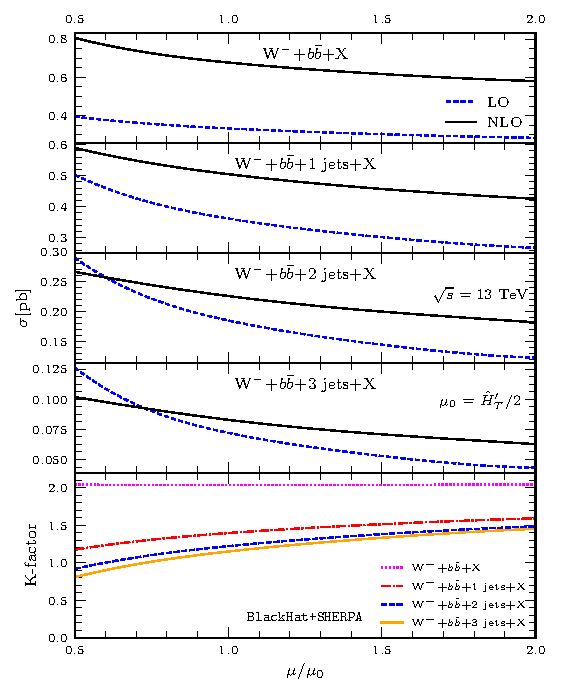
\includegraphics[clip,scale=0.88]{plots/scale_dependence_Wmbb}
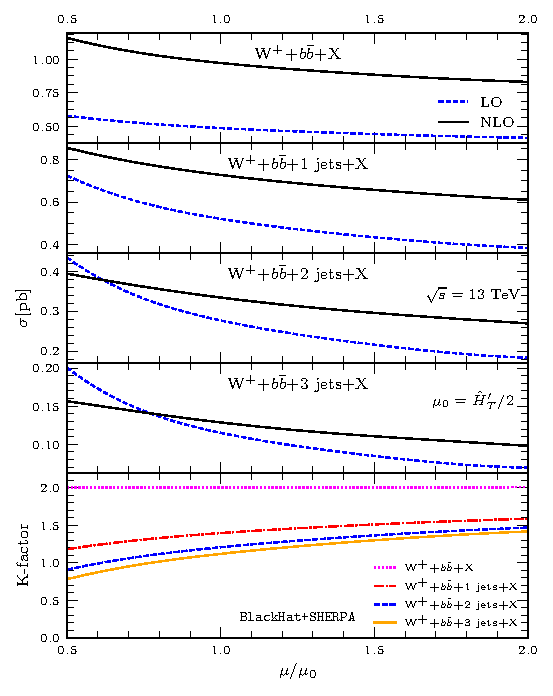
\includegraphics[clip,scale=0.88]{plots/scale_dependence_Wpbb}
\end{centering}
\caption{Renormalization- and factorization-scale dependence of total cross
  sections for \Wbbm$+0,1,2,3$-jet$+X$ production to the left and
\Wbbp$+0,1,2,3$-jet$+X$ production to the right. We use the central scale $\mu_0=\mu_{\textrm r}=\mu_{\textrm f}=\HTpartonicp/2$. In the upper four panels, we show the dependence of LO (dashed blue line) and
  NLO (solid black line) predictions on the scale $\mu$. The lower panel shows
  the respective $K$-factor (ratio of NLO/LO).}
\label{fig_Wjets_sdep}
\end{figure}
%%%%%%%%%%%%%%%%%%%%%%%%%%%%%%%%%%%%%%%

The dynamical scale $\HTpartonicp/2$ increases on average monotonically with
multiplicity. For vector boson production in association with massless
jets, this scale choice has been observed to produce relatively stable NLO results over a wide range of kinematical
configurations relevant to the LHC and future
colliders~\cite{BH:W3jPRL,BH:W4j,BH:W5j,Mangano:2016jyj}. For the LHC in
particular, it has been observed that for massless jet production the scale
$\HTpartonicp/2$ typically produced NLO cross sections lying on the locus of the
scale-dependence curves. Contrary to that we observe that for \Wbbn{} production, the
NLO cross section at the central scale appears consistently on the right of the
scale-dependence plateau. We assert, in particular considering the
similarities of the massive and massless results studied in
Section~\ref{sec:bmass}, that this difference has little to do with the presence
of a massive jet and it is actually due to the type of
subprocesses contributing. In light-jet production the dominant
subprocesses are the ones with a single fermion line. In the case of
\Wbbn{} production in turn, the dominant subprocesses are those with
two fermionic lines (the ones with most gluons involved).

%pt leading bjet
%%%%%%%%%%%%% FIGURE %%%%%%%%%%%%%%%%%%
\begin{figure}[t]
\centering
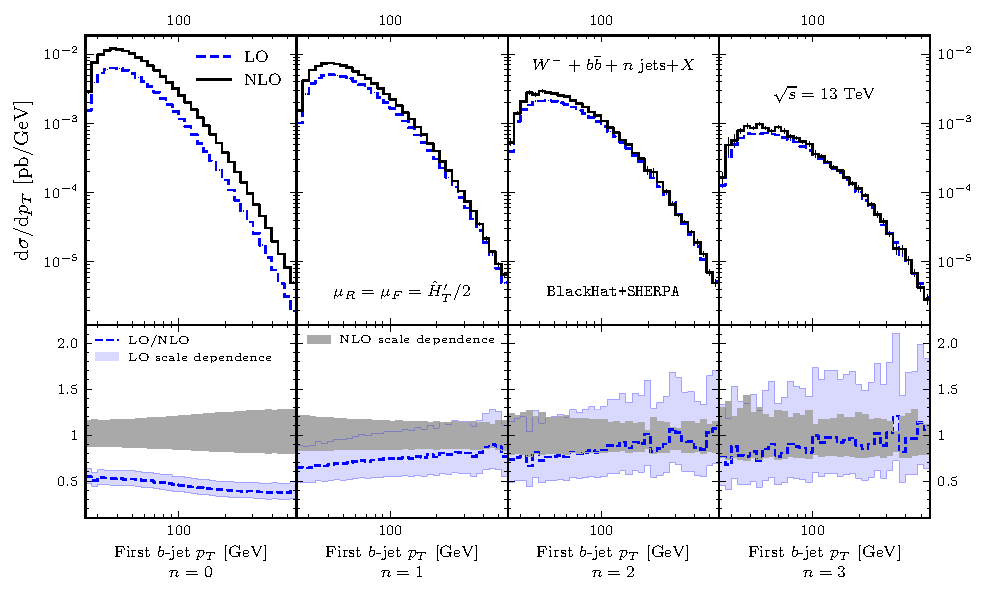
\includegraphics[clip,scale=1]{plots/ptleading}
  \caption{The $\pT$ distributions of the leading $b$ jet (ordered by $p_T$) in inclusive \Wbbm$+0,1,2,3$-jet
    production at the LHC at $\sqrt{s}=13$~TeV. Light
    jet multiplicity increases from left to right. In the upper panels the
    dashed (blue) line shows the LO result and the solid (black) line the NLO
    result. Vertical thin lines show the statistical error from the numerical
    integration. In the bottom panels we show the scale-dependence bands
    normalized to the NLO result, in blue for LO and gray for NLO.}
  \label{fig_Wmnjpt}
\end{figure}
%%%%%%%%%%%%%%%%%%%%%%%%%%%%%%%%%%%%%%%

%pt subleading bjet
%%%%%%%%%%%%% FIGURE %%%%%%%%%%%%%%%%%%
\begin{figure}[t]
\centering
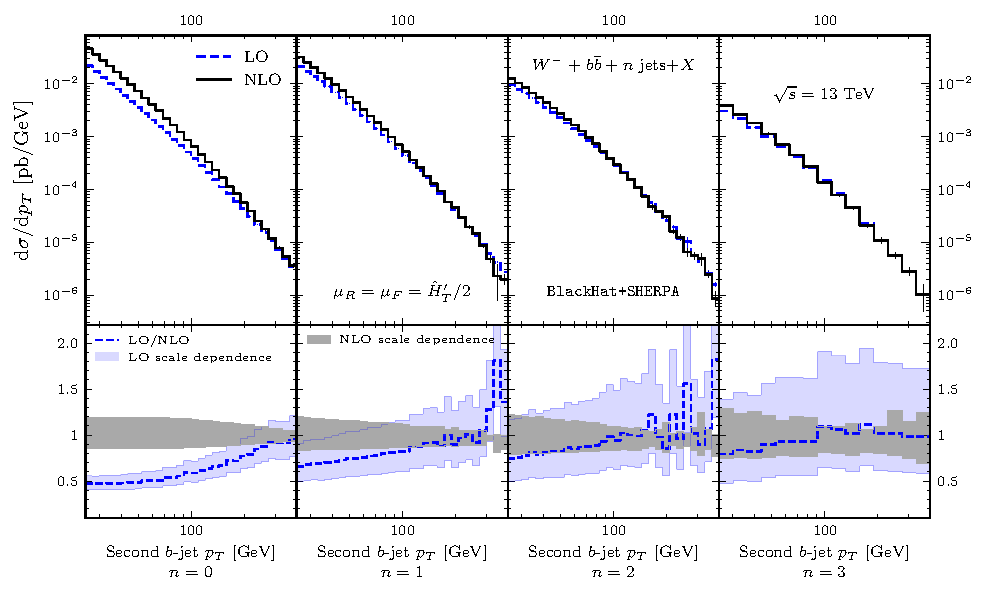
\includegraphics[clip,scale=1]{plots/ptsubleading}
  \caption{The $\pT$ distributions of the subleading $b$ jet (ordered by $p_T$) in inclusive \Wbbm$+0,1,2,3$-jet
    production at the LHC at $\sqrt{s}=13$~TeV. Format as in \fig{fig_Wmnjpt}.}
  \label{fig_Wmnjpt2}
\end{figure}
%%%%%%%%%%%%%%%%%%%%%%%%%%%%%%%%%%%%%%%



\subsection{Differential Cross Sections}
\label{diffxsw}

This section is devoted to the study of NLO results for several differential
distributions and we will thereby highlight the impact of NLO QCD corrections on fixed-order predictions over phase space. The structure of corrections is similar for the $W^\pm$ species and we will in general only show results for one of them.

In \figs{fig_Wmnjpt}{fig_Wmnjpt2} we show the jet-$p_T$ spectra of leading
and subleading $b$ jets (ordered by $p_T$) respectively, for inclusive
\Wbbm{} production in association with $n=0,1,2,3$ jets. In the upper panel of the
figures, we show LO and NLO distributions as dashed (blue) and solid (black)
lines respectively. The bottom panels show the scale-dependence bands
normalized to the central NLO result (LO in blue and NLO in gray). Numerical
integration errors for each bin are shown as thin vertical lines (when visible).
We show all distributions in this section in a similar manner.

We observe that the NLO corrections have structure beyond the $K$-factors studied at
the level of total cross sections in the previous subsection. In most of the $p_T$ distributions of $b$ jets, shape differences
are present between LO and NLO results. Typically, the LO predictions become harder. This trend is reduced with light-jet multiplicity and for the highest-multiplicity process considered, \Wbbnj[3]{} production,
the LO/NLO shape difference
is reduced. An exception to this observation is the leading
$b$ jet $p_T$ in \Wbb{} production. As expected, the scale dependence of NLO
results is reduced compared to LO results (apart from \Wbb{}, as
discussed for total cross sections) and in the high-multiplicity samples, NLO results
lie inside LO bands. This confirms the relatively good perturbative control for the high-multiplicity samples.

%Softest light-jet PT
%%%%%%%%%%%%% FIGURE %%%%%%%%%%%%%%%%%%
\begin{figure}[t]
\centering
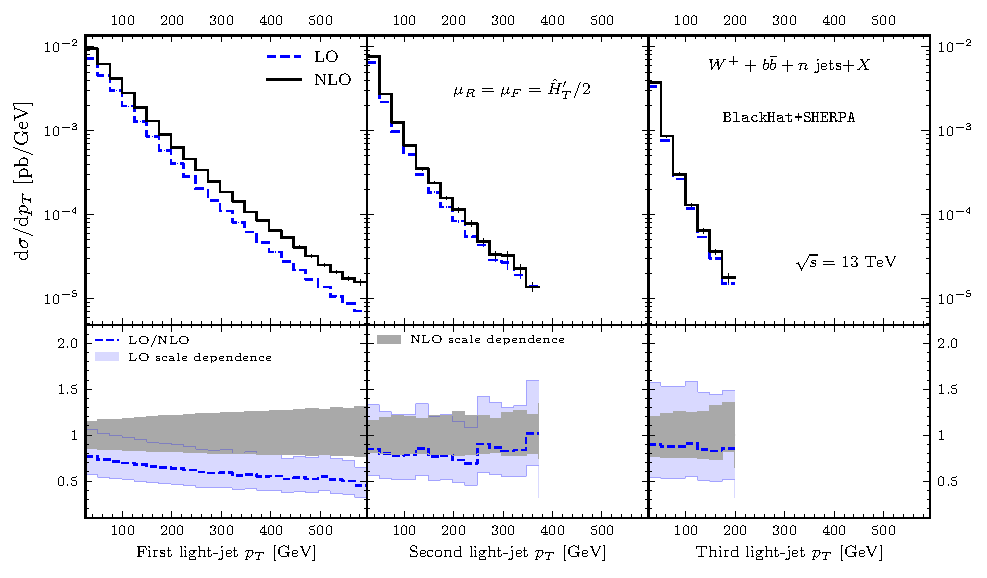
\includegraphics[clip,scale=1]{plots/softestpt}
  \caption{The $\pT$
distributions of the softest light jets in inclusive \Wbbp$+1,2,3$-jet production.
Format as in \fig{fig_Wmnjpt}.}
  \label{fig_Wmnjptlight}
\end{figure}
%%%%%%%%%%%%%%%%%%%%%%%%%%%%%%%%%%%%%%%

In \fig{fig_Wmnjptlight} we show the $p_T$ distribution of the softest light jet in
inclusive \Wbbp{}$+1,2,3$-jet production.
%, which are experimentally relevant since they are quite sensitive to the jet-energy scale. 
We observe a reduction of the scale
sensitivity with the inclusion of QCD corrections, with LO
and NLO bands overlapping. The quantum corrections for these
distributions are rather flat. This feature is similar to
observations for softest jet $p_T$ distributions in $W+n$-light-jet
production.


%HT jet / hadronic
%%%%%%%%%%%%% FIGURE %%%%%%%%%%%%%%%%%%
\begin{figure}[ht]
\centering
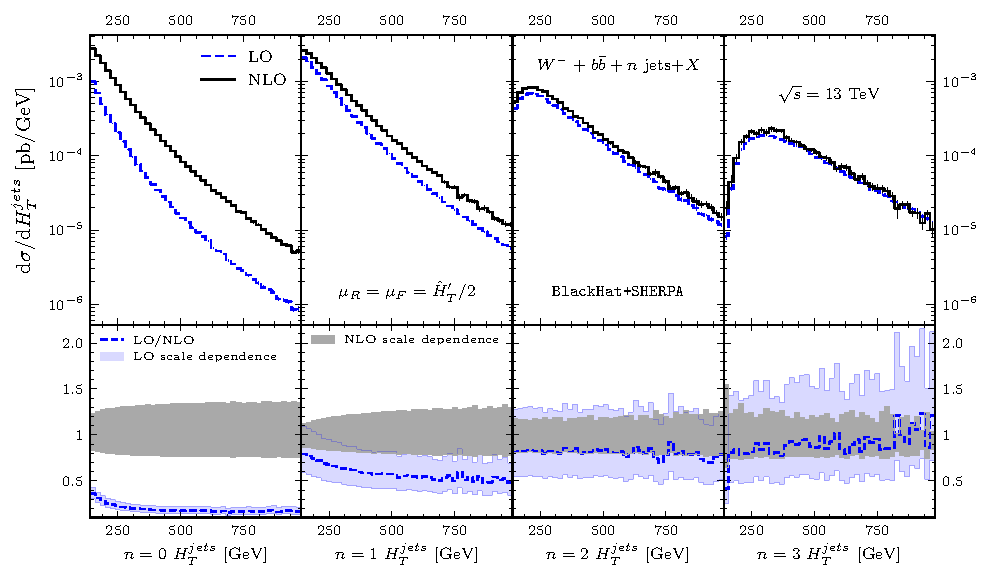
\includegraphics[clip,scale=1.0]{plots/htjets.pdf}
  \caption{Distributions of total transverse jet energy
    $H_T^{jets}$ of light and $b$ jets for inclusive \Wbbm$+0,1,2,3$-jet
    production at the LHC at $\sqrt{s}=13$~TeV. Format as in \fig{fig_Wmnjpt}.}
  \label{fig_Wmnjht}
\end{figure}
%%%%%%%%%%%%%%%%%%%%%%%%%%%%%%%%%%%%%%%

The total hadronic activity in a detector is an interesting observable
for many BSM scenarios, as well as for
experimental studies at hadron colliders. In \fig{fig_Wmnjht} we show distributions in
this observable, including all hadronic activity from light and $b$ jets in
\Wbbm$+0,1,2,3$-jet production. As we would expect from previous
discussions, strikingly large and phase-space dependent NLO
corrections appear for \Wbb{}. Interestingly, a remnant of these large effects remains in \Wbbnj[1]{}
production in this observable. For \Wbbnj[1]{}, the QCD corrections are
not as large as for \Wbb{}, but at around 1~TeV for $H_T^{jets}$, we
still observe a differential $K$-factor reaching two, with the shape difference ending at about 400~GeV. The large-multiplicity processes on the other hand show much less
structure. In particular, enhancements due to soft $W$ emission are present already at LO in this case.

%dR first b-jet / charged lepton
%%%%%%%%%%%%% FIGURE %%%%%%%%%%%%%%%%%%
\begin{figure}[ht]
\centering
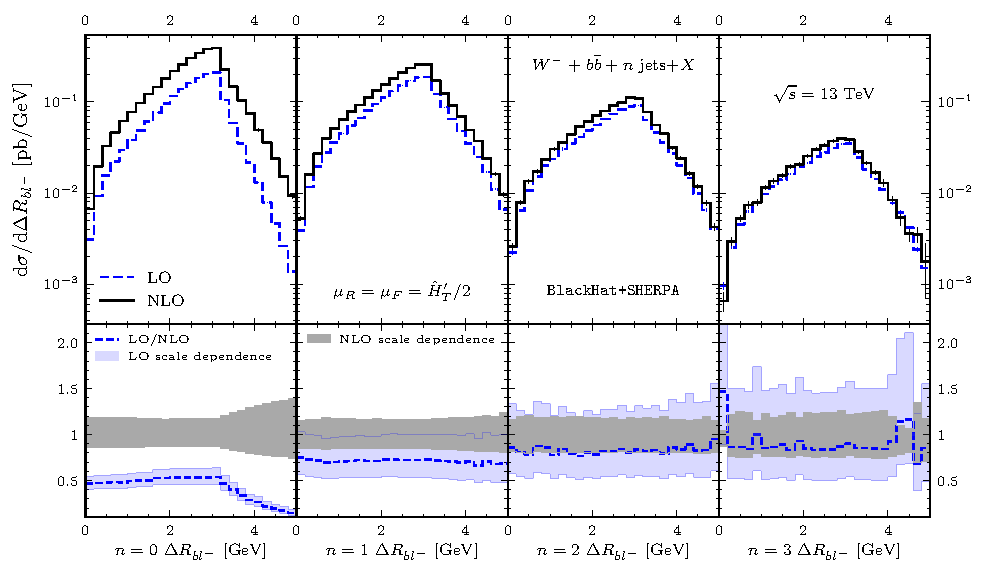
\includegraphics[clip,scale=1.0]{plots/drbl.pdf}
  \caption{Distributions in the $\Delta R_{bl^-}$ separation between first
    $b$ jet (ordered in $p_T$) and charged lepton for inclusive \Wbbm$+n$ jets
    production. Format as in \fig{fig_Wmnjpt}.}
  \label{fig_Wmnjdrbl}
\end{figure}
%%%%%%%%%%%%%%%%%%%%%%%%%%%%%%%%%%%%%%%


Lastly, we show in \fig{fig_Wmnjdrbl} distributions
in the $\Delta R$ separation between first $b$ jet and charged
lepton $l^-$. Most of the angular variables that we studied are
similar to this one, showing little structure in the QCD corrections. However, we find an effect when a certain kinematic constraint is
imposed at LO and released by the QCD corrections, as visible on the left most plots of \fig{fig_Wmnjdrbl}. In the LO $\Delta R_{bl^-}$ distribution for \Wbbm{} production, the parent $W$
and gluon that give rise to the leptons and $b$ jets respectively are produced with $\Delta
\phi$ (the difference in azimuthal angle) equal to $\pi$. Also, the $\Delta \eta$
distribution peaks at around zero and decreases monotonically. The
resulting $\Delta R_{bl^-}$ distribution thus has the feature of a
sharply decaying distribution at LO. This constraint is lifted at NLO by real corrections. Also the higher-multiplicity cases of \Wbb$+1,2,3$-jet production do not exhibit a similar feature.

\section{Backgrounds to $HW$ Production}
\label{sec:hw}

Many of the properties of the Higgs boson have been studied at the LHC, and so far all measurements appear in good agreement with the
predictions of the SM (see for
example Ref.~\cite{Khachatryan:2016vau}). However, it will be important to further constrain the strength of the Yukawa coupling
$y_b$ of the Higgs
boson to $b$ quarks, given that a Higgs boson with mass $M_h$ around 125 GeV decays about half of the time into a $b\bar b$ pair. In the main
production channel of the Higgs, through gluon-gluon fusion, one faces
a huge background from pure QCD $b\bar b$ production. Therefore,
considering the associated $H(\rightarrow b\bar{b})W$ production can help solidify the evidence for the Higgs decaying to $b$ quarks \cite{ATLAS:hbb2017}. Important for this approach is of course that irreducible backgrounds with the same signature, such as \Wbb{} production in the SM, can be kept under control. We aim to contribute
to this quest with the predictions provided in this section.


In this section, we study three observables that are important for $HW$
analyses, in the context of our high-multiplicity results: On the one hand, $p_T^{b\bar b}$ and $M_{b\bar b}$, which are associated to the $b\bar
b$ system and, when producing a Higgs, are associated with the $p_T$ distributions of the
Higgs and the mass of the
Higgs. Furthermore, we study $p_T^W$, which helps to characterize the
accompanying $W$ boson. At high energies and multiplicities, resonant top contributions, as studied for example in~\cite{Denner:2017kzu}, are equally present. In the context of $HW$ production
the focus is on the non-resonant backgrounds, where top contributions are also sizable. They can be of similar order to the contributions presented here, even though they are formally suppressed by powers of $\alpf/\alps$. A more systematic study of $HW$ backgrounds should thus include non-resonant top contribution, which we leave to future work.

%pt(bb) 
%%%%%%%%%%%%% FIGURE %%%%%%%%%%%%%%%%%%
\begin{figure}[t]
\centering
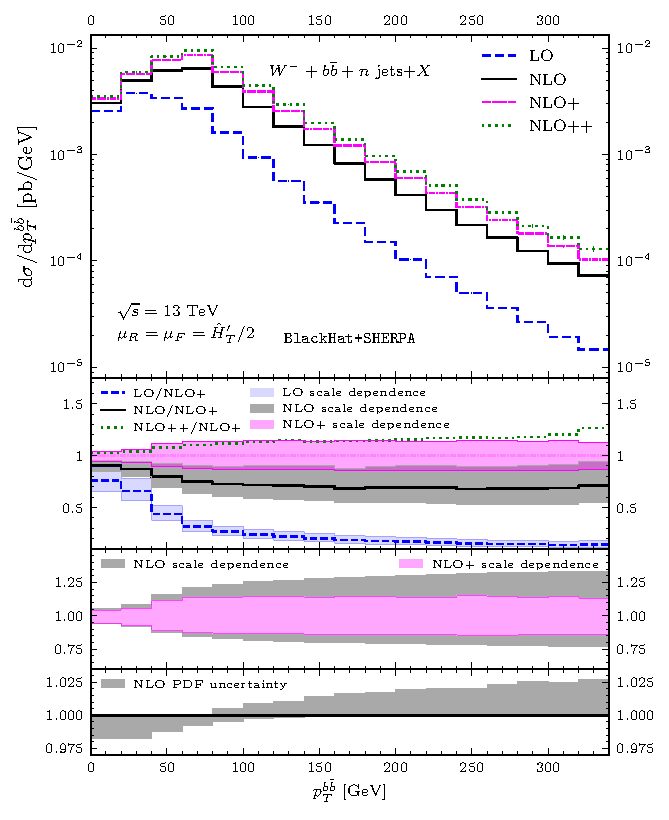
\includegraphics[clip,scale=1]{plots/excl_ptbb_v4}
\caption{The $p_T$ distribution of the $b\bar{b}$ system in inclusive \Wbbm{} production,
    computed at LO (dashed blue line) and NLO (solid black line) as well as
    by employing the exclusive sums NLO+ (dashed-dot magenta line)
    and NLO++ (dotted green line). The second panel shows scale dependence bands normalized by NLO+,
    and the third panel shows results normalized by the corresponding
    central value. The bottom panel shows the associated PDF uncertainties
    normalized to our NLO results.}
  \label{fig_Wmnjptbb}
\end{figure}
%%%%%%%%%%%%%%%%%%%%%%%%%%%%%%%%%%%%%%%

We have seen in this chapter and it has been understood since a long time that NLO QCD correction to \Wbb{} production have large contributions associated to
processes with an extra light jet. Previous approaches used
exclusive results in the number of light jets~\cite{FebresCordero:2006sj}, which explicitly vetoed
events with extra jets. This prescription however suffers from its sensitivity
associated to the $p_T^{\textrm veto}$ cut~\cite{Tackmann:2012bt}. We choose to follow a different approach. Instead of imposing a veto cut to stabilize the predictions, we
effectively replace the extra light-jet contributions to generic observables,
which are effectively LO, by their corresponding results including NLO QCD
corrections. In higher-order corrections these contributions are naturally
added and our predictions will be outdated once NNLO predictions for \Wbb{} production become available in the future.

We apply the `exclusive sums' technique which was studied
in~\cite{ESums}. In particular, this technique is expected to be of benefit when
tree-like contribution, with an extra light jet, to NLO corrections are rather
large. Notice that in measurements of $W$+light jets some of the predictions
from exclusive sums have been compared to LHC data, see for
example~\cite{Aad:2014qxa,ATLAS:ratio2017}, usually in the context of
$W+1$-jet production. By now those computations are outdated, given the recent NNLO QCD calculation
presented in Ref.~\cite{Boughezal:2015dva}. Other approaches studied to get more realistic predictions for the comparison to LHC data are the
application of a parton-shower \cite{Luisoni:2015mpa}, or using a
matched and merged version for example with the MEPS@NLO \cite{Hoeche:2012yf} or FxFx technique \cite{Frederix:2012ps}.

%pt(W) 
%%%%%%%%%%%%% FIGURE %%%%%%%%%%%%%%%%%%
\begin{figure}[t]
\centering
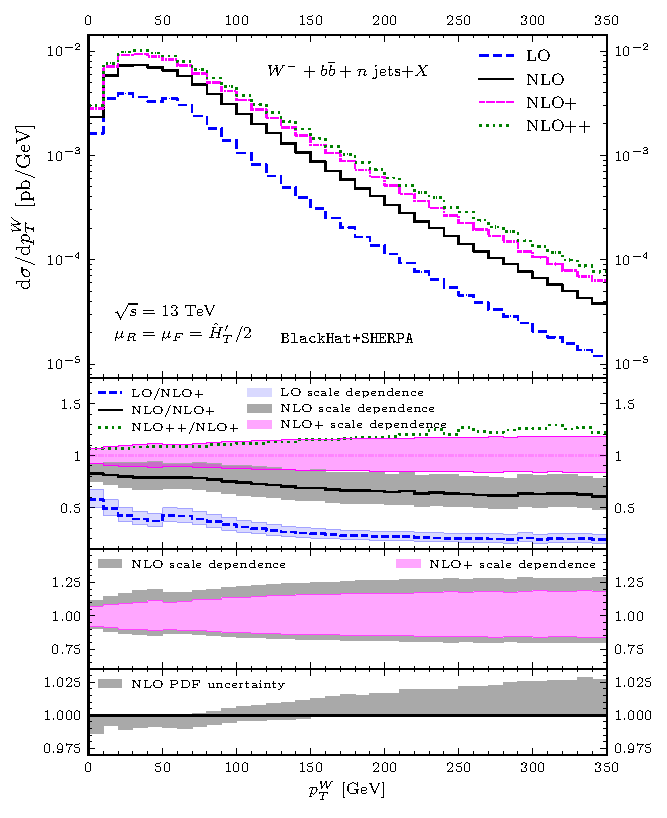
\includegraphics[clip,scale=1]{plots/excl_ptw_v4}
  \caption{The $p_T$ of the $W$ boson in inclusive \Wbbm{} production. Format as in \fig{fig_Wmnjptbb}.}
  \label{fig_Wmnjptw}
\end{figure}
%%%%%%%%%%%%%%%%%%%%%%%%%%%%%%%%%%%%%%%

In this section, we focus on predictions for \Wbb$+X$ production. We
denote fixed-order
results for those as usual with the labels LO and
NLO. Furthermore, we employ exclusive sums as defined in
Eq.~\eqref{eq:excsums}, for which we use labels NLO+ and NLO++. The latter serves as a proxy for the size of even
higher-order corrections and thus to estimate the theoretical uncertainty.

In order to characterize theoretical uncertainties in a more complete way, we also explore PDF uncertainties associated to the
observables under consideration. To that end, we estimate the
associated PDF uncertainties from the error sets of the pseudo-PDF set
\texttt{PDF4LHC15\_nlo\_nf4\_30}~\cite{Butterworth:2015oua}, which have been produced as a by-product of the major PDF sets according to the so
called `PDF4LHC' recommendations. Since the PDF error we find are
small compared to
other theoretical uncertainties, we do not go beyond this
restricted error set for our estimations. Further uncertainties are
associated to the value of $m_b$ and $\alps$, but those are expected to
be rather small compared to missing higher-order
corrections.


%Mbb 
%%%%%%%%%%%%% FIGURE %%%%%%%%%%%%%%%%%%
\begin{figure}[t]
\centering
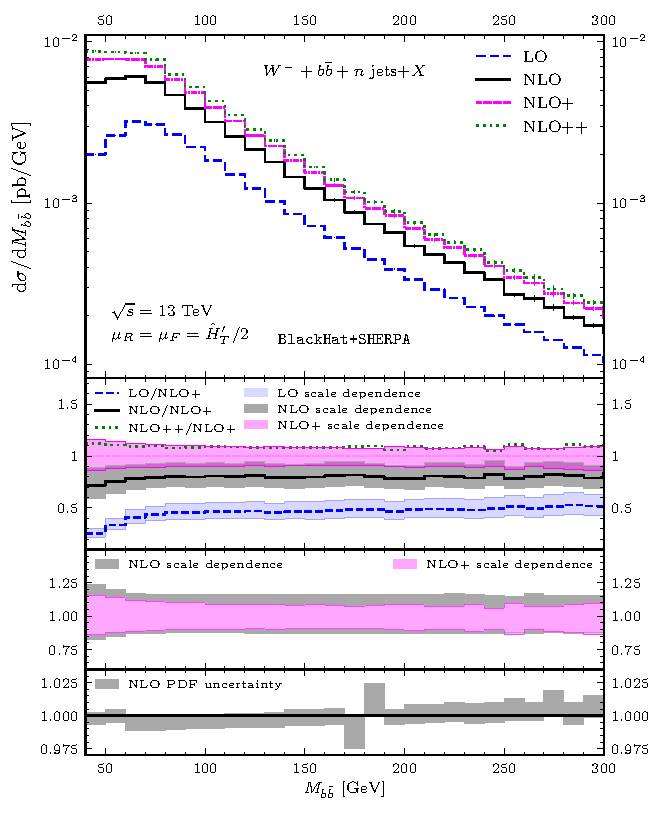
\includegraphics[clip,scale=1]{plots/excl_mbb_v4}
  \caption{The invariant mass of the $b\bar b$ system in inclusive \Wbbm{} production. Format as in \fig{fig_Wmnjptbb}.}
  \label{fig_Wmnjmbb}
\end{figure}
%%%%%%%%%%%%%%%%%%%%%%%%%%%%%%%%%%%%%%%

In \fig{fig_Wmnjptbb}, we show the distribution of transverse momentum of
the $b\bar b$ system. The upper panel contains all our predictions, that is the central
NLO+ prediction as well as LO, NLO and NLO++. In the second panel, we
show the corresponding scale-dependence bands at LO, NLO and NLO+, all normalized by NLO+, as well as the central value for
NLO++. In the third panel we show the scale-dependence bands at
NLO and NLO+, normalized by the respective central value. Lastly, in
the bottom panel, we show the PDF uncertainties, which are below
2\% for the range of $p_T^{b\bar b}$ shown (we normalize the PDF
uncertainties by the NLO result). The NLO+ predictions have smaller scale-dependence bands at the level
of 13\%, which is a reduction compared to those of the fixed-order
NLO result. No adequate prediction is given by the LO result. The NLO
and NLO+ bands overlap, but show a difference in shape, particularly
at low values of $p_T^{b\bar b}$. The estimation of higher-order corrections through scale variations and by the NLO++
results are of the same order of magnitude.



We observes the release of a kinematical constraint at NLO for the
$p_T^{b\bar b}$ observable. At LO, the massive $b$-quark pair
originates in a gluon splitting and $p_T^{b\bar b}$ and
$p_T^W$ are back-to-back. At NLO, real radiation emission relaxes this
constraint and yields large corrections, due to a soft enhancement for low $p_T^W$. The release of this constraint together with the opening of a gluon-initiated channel give rise to a giant $K$-factor~\cite{Rubin:2010xp}. The kinematical constraint in \Wbb{} is
similar to those appearing in $V+1$ light jet (see e.g.\ Refs.~\cite{BH:W3jPRL,BH:W4j,BH:W5j}). The characteristics of
the NLO results for \Wbb{} production are thus expected~\cite{Catani:1997xc}.


In \fig{fig_Wmnjptw}, we show the distribution in the transverse
momentum of the vector boson $p_T^W$ in the same format. We find similar results as for $p_T^{b\bar b}$: the NLO+ uncertainty
estimation is marginally
overlapping with the NLO predictions and has a scale sensitivity of the order
of the NLO++ predictions. We estimate theoretical uncertainties to about 17\% in the
range of $p_T^W$ shown (as compared to the 25\% of the NLO
results). As before, PDF uncertainties are
subleading, appearing at 3\% and below.

The last observable we show in \fig{fig_Wmnjmbb} is the distribution in $M_{b\bar b}$, which exhibits similar features to the observables
studied previously in this section. Here, we estimate the uncertainties associated with scale
sensitivity and missing higher-order effects to about 10\% or slightly
smaller. The PDF uncertainties are tiny, being at 1\% or smaller. 


